\RequirePackage{luatex85}
\documentclass[tikz]{standalone}
% Default preamble
\usepackage{pgfplots}
\pgfplotsset{compat=newest}
\usepgfplotslibrary{groupplots}
\usepgfplotslibrary{polar}
\usepgfplotslibrary{smithchart}
\usepgfplotslibrary{statistics}
\usepgfplotslibrary{dateplot}
\usepgfplotslibrary{ternary}
\usepackage[T1]{fontenc}
\usepackage{lmodern}
\begin{document}
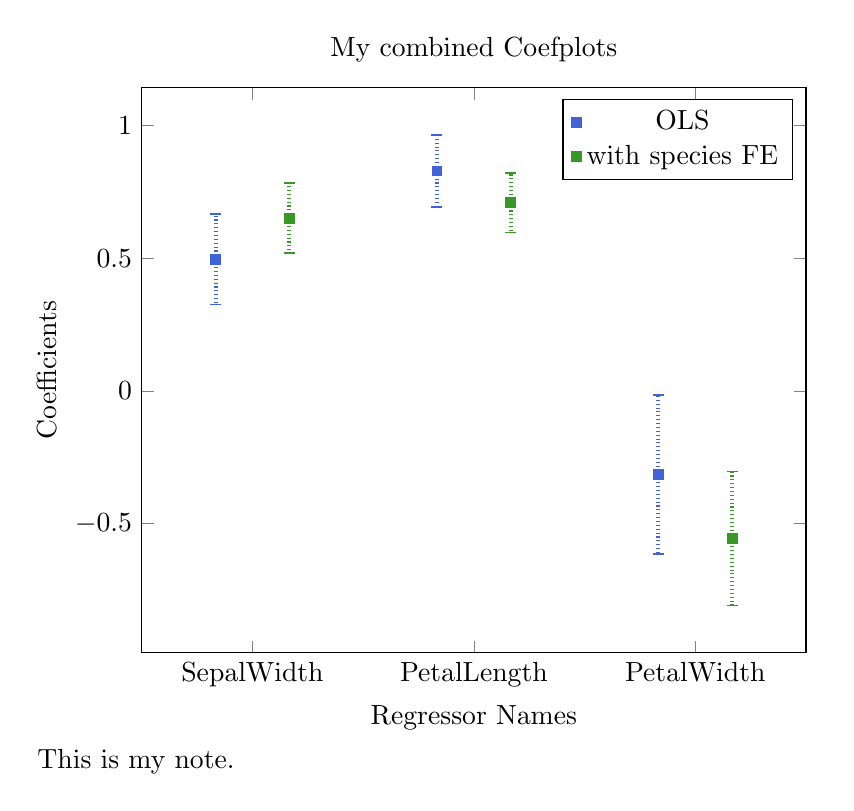
\begin{tikzpicture}
\begin{axis}[title={My combined Coefplots}, title style={}, xlabel={Regressor Names}, xlabel style={}, ylabel={Coefficients}, ylabel style={}, xticklabel style={}, yticklabel style={}, width={240pt}, height={204pt}, legend style={}, symbolic x coords={SepalWidth,PetalLength,PetalWidth}, xtick={SepalWidth,PetalLength,PetalWidth}, xmin={{[normalized]-0.5}}, xmax={{[normalized]2.5}}, scale only axis]
    \addplot[only marks, mark={square*}, mark options={mark size={1.75pt}, line width={0pt}, fill={rgb,255: red, 64; green, 99; blue, 216}, fill opacity={1}, draw={rgb,255: red, 64; green, 99; blue, 216}, draw opacity={1}}, error bars/error mark={|}, error bars/error mark options={mark size={2.0pt}, solid, line width={0.6pt}, fill={rgb,255: red, 64; green, 99; blue, 216}, fill opacity={1}, draw={rgb,255: red, 64; green, 99; blue, 216}, draw opacity={1}}, error bars/error bar style={draw={rgb,255: red, 64; green, 99; blue, 216}, draw opacity={1}, densely dotted, line width={1.5pt}}, draw={rgb,255: red, 64; green, 99; blue, 216}, draw opacity={1}, line width={0.5pt}, error bars/y dir={both}, error bars/y explicit, x filter/.code={{\pgfmathadd{\pgfmathresult}{-0.16666666666666666}}}]
        coordinates {
            (SepalWidth,0.4958889383885524) +- (0,0.17011)
            (PetalLength,0.8292439122348061) +- (0,0.13544)
            (PetalWidth,-0.31515517332647486) +- (0,0.29883)
        }
        ;
    \addlegendentry {OLS}
    \addplot[only marks, mark={square*}, mark options={mark size={1.75pt}, line width={0pt}, fill={rgb,255: red, 56; green, 152; blue, 38}, fill opacity={1}, draw={rgb,255: red, 56; green, 152; blue, 38}, draw opacity={1}}, error bars/error mark={|}, error bars/error mark options={mark size={2.0pt}, solid, line width={0.6pt}, fill={rgb,255: red, 56; green, 152; blue, 38}, fill opacity={1}, draw={rgb,255: red, 56; green, 152; blue, 38}, draw opacity={1}}, error bars/error bar style={draw={rgb,255: red, 56; green, 152; blue, 38}, draw opacity={1}, densely dotted, line width={1.5pt}}, draw={rgb,255: red, 56; green, 152; blue, 38}, draw opacity={1}, line width={0.5pt}, error bars/y dir={both}, error bars/y explicit, x filter/.code={{\pgfmathadd{\pgfmathresult}{0.16666666666666666}}}]
        coordinates {
            (SepalWidth,0.65083715931332) +- (0,0.13172)
            (PetalLength,0.7091319591367369) +- (0,0.1121)
            (PetalWidth,-0.5564826601670136) +- (0,0.25208)
        }
        ;
    \addlegendentry {with species FE}
\end{axis}
\newdimen\notewidth
                    \pgfextractx{\notewidth}{\pgfpointdiff{\pgfpointanchor{current bounding box}{west}}
                    {\pgfpointanchor{current bounding box}{east}}}\draw node[text width={\the\notewidth}, anchor={north west}, at={(current axis.outer south west)}, align={left}] {This is my note.};
\end{tikzpicture}
\end{document}
